\documentclass[tikz,border=6pt]{standalone}
\usepackage{amsmath,amssymb}
\usepackage{xcolor}
\definecolor{accent}{HTML}{A13D2C}
\definecolor{accent2}{HTML}{2B5F6B}
\definecolor{muted}{HTML}{5A564F}
\definecolor{linecol}{HTML}{D8D2C4}
\definecolor{astroblue}{HTML}{1B4F72}
\usetikzlibrary{calc}
% Poisson probabilities P(n) = nbar^n e^{-nbar}/n! (stems or dots) and the Gaussian of mean nbar and
% variance nbar (dashed), for nbar = 0.1, 1, 10, 100, 1000.
% The P(n) values were computed exactly in Wolfram:
%   f[m_,ns_] := Table[{n, N[m^n Exp[-m]/n!, 12]}, {n, ns}]
%   f[1/10,Range[0,3]], f[1,Range[0,8]], f[10,Range[0,25]], f[100,Range[64,136,2]], f[1000,Range[880,1120,6]]
% The Gaussian curves are computed by TikZ from their formula.
\newcommand{\PW}{4.4}  % panel width (cm)
\newcommand{\PH}{2.5}  % panel height (cm)
% #1,#2 panel origin (cm); #3,#4 n range; #5 y maximum; #6 nbar; #7 label of nbar; #8 x ticks; #9 y tick
\newcommand{\panel}[9]{%
  \begin{scope}[shift={(#1,#2)}]
    \draw[muted] (0,0) -- (\PW,0);
    \draw[muted] (0,0) -- (0,\PH);
    \pgfmathsetmacro{\xu}{\PW/(#4-#3)}
    \pgfmathsetmacro{\yu}{\PH/#5}
    \foreach \t in {#8} {
      \pgfmathsetmacro{\xt}{(\t-#3)*\xu}
      \draw[muted] (\xt,0) -- (\xt,-0.07) node[below] {\scriptsize $\t$};
    }
    \pgfmathsetmacro{\yt}{#9*\yu}
    \draw[muted] (0,\yt) -- (-0.07,\yt) node[left] {\scriptsize $#9$};
    \node[anchor=north east] at (\PW,\PH) {\small $\bar n=#7$};
  \end{scope}%
}
\begin{document}
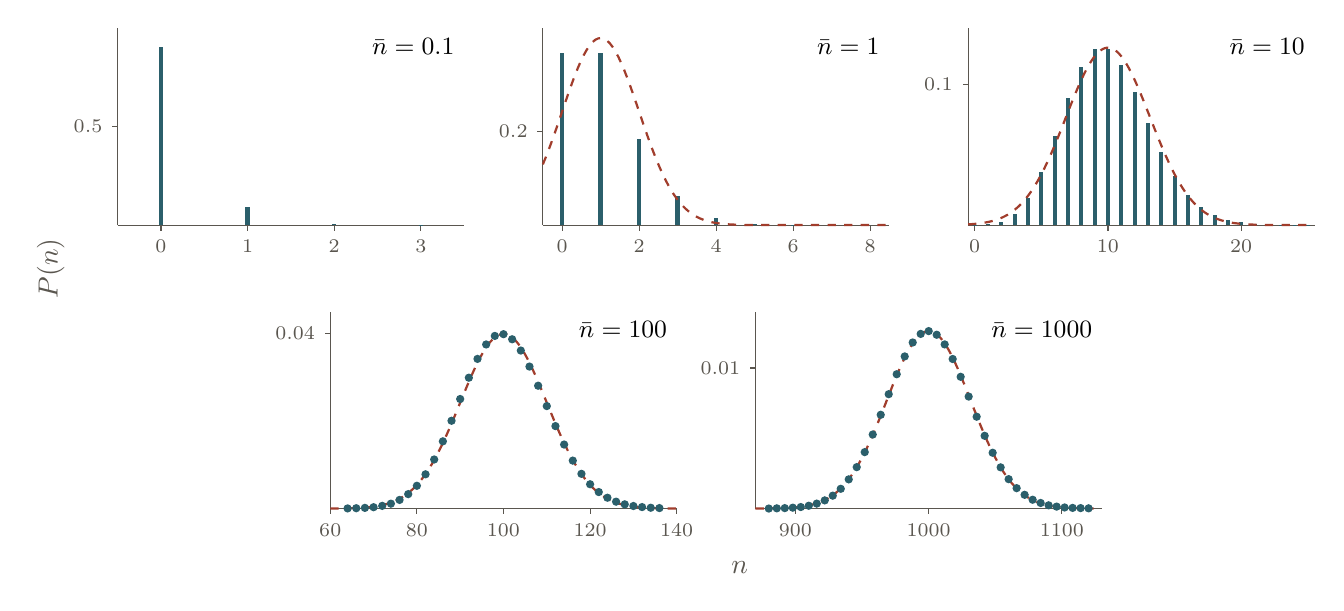
\begin{tikzpicture}
  % ---------------- nbar = 0.1 ----------------
  \panel{0}{3.6}{-0.5}{3.5}{1.0}{0.1}{0.1}{0,1,2,3}{0.5}
  \begin{scope}[shift={(0,3.6)}, x={(\PW cm/4,0)}, y={(0,\PH cm/1.0)}, xshift={0.5*\PW cm/4}]
    \foreach \n/\p in {0/0.904837, 1/0.0904837, 2/0.00452419, 3/0.000150806}
      { \draw[accent2, line width=1.6pt] (\n,0) -- (\n,\p); }
  \end{scope}
  % ---------------- nbar = 1 ----------------
  \panel{5.4}{3.6}{-0.5}{8.5}{0.42}{1}{1}{0,2,4,6,8}{0.2}
  \begin{scope}[shift={(5.4,3.6)}, x={(\PW cm/9,0)}, y={(0,\PH cm/0.42)}, xshift={0.5*\PW cm/9}]
    \foreach \n/\p in {0/0.36788, 1/0.36788, 2/0.18394, 3/0.06131, 4/0.01533, 5/0.00307, 6/0.00051, 7/0.00007, 8/0.000009}
      { \draw[accent2, line width=1.6pt] (\n,0) -- (\n,\p); }
    \draw[accent, dashed, line width=0.8pt, domain=-0.5:8.5, samples=120] plot (\x, {exp(-(\x-1)^2/2)/sqrt(2*pi)});
  \end{scope}
  % ---------------- nbar = 10 ----------------
  \panel{10.8}{3.6}{-0.5}{25.5}{0.14}{10}{10}{0,10,20}{0.1}
  \begin{scope}[shift={(10.8,3.6)}, x={(\PW cm/26,0)}, y={(0,\PH cm/0.14)}, xshift={0.5*\PW cm/26}]
    \foreach \n/\p in {0/0.00005, 1/0.00045, 2/0.00227, 3/0.00757, 4/0.01892, 5/0.03783, 6/0.06306, 7/0.09008, 8/0.11260, 9/0.12511, 10/0.12511, 11/0.11374, 12/0.09478, 13/0.07291, 14/0.05208, 15/0.03472, 16/0.02170, 17/0.01276, 18/0.00709, 19/0.00373, 20/0.00187, 21/0.00089, 22/0.00040, 23/0.00018, 24/0.00007, 25/0.00003}
      { \draw[accent2, line width=1.4pt] (\n,0) -- (\n,\p); }
    \draw[accent, dashed, line width=0.8pt, domain=-0.5:25.5, samples=150] plot (\x, {exp(-(\x-10)^2/20)/sqrt(20*pi)});
  \end{scope}
  % ---------------- nbar = 100 ----------------
  \panel{2.7}{0}{60}{140}{0.045}{100}{100}{60,80,100,120,140}{0.04}
  \begin{scope}[shift={(2.7,0)}, x={(\PW cm/80,0)}, y={(0,\PH cm/0.045)}, xshift={-60/80*\PW cm}]
    \draw[accent, dashed, line width=0.8pt, domain=60:140, samples=150] plot (\x, {exp(-(\x-100)^2/200)/sqrt(200*pi)});
    \foreach \n/\p in {64/0.00003, 66/0.00007, 68/0.00015, 70/0.00031, 72/0.00061, 74/0.00112, 76/0.00197, 78/0.00329, 80/0.00520, 82/0.00783, 84/0.01122, 86/0.01536, 88/0.02006, 90/0.02504, 92/0.02991, 94/0.03421, 96/0.03751, 98/0.03946, 100/0.03986, 102/0.03869, 104/0.03612, 106/0.03245, 108/0.02808, 110/0.02342, 112/0.01884, 114/0.01463, 116/0.01096, 118/0.00794, 120/0.00556, 122/0.00377, 124/0.00247, 126/0.00157, 128/0.00096, 130/0.00058, 132/0.00033, 134/0.00019, 136/0.00010}
      { \fill[accent2] (\n,\p) circle[radius=1.5pt]; }
  \end{scope}
  % ---------------- nbar = 1000 ----------------
  \panel{8.1}{0}{870}{1130}{0.014}{1000}{1000}{900,1000,1100}{0.01}
  \begin{scope}[shift={(8.1,0)}, x={(\PW cm/260,0)}, y={(0,\PH cm/0.014)}, xshift={-870/260*\PW cm}]
    \draw[accent, dashed, line width=0.8pt, domain=870:1130, samples=150] plot (\x, {exp(-0.5*((\x-1000)/31.6228)^2)/79.2665});
    \foreach \n/\p in {880/0.0000074, 886/0.000016, 892/0.000031, 898/0.000061, 904/0.000113, 910/0.000203, 916/0.000349, 922/0.000578, 928/0.000919, 934/0.001407, 940/0.002072, 946/0.002938, 952/0.004009, 958/0.005268, 964/0.006668, 970/0.008130, 976/0.009551, 982/0.010815, 988/0.011806, 994/0.012426, 1000/0.012615, 1006/0.012353, 1012/0.011672, 1018/0.010643, 1024/0.009368, 1030/0.007961, 1036/0.006533, 1042/0.005178, 1048/0.003965, 1054/0.002933, 1060/0.002097, 1066/0.001450, 1072/0.000969, 1078/0.000626, 1084/0.000391, 1090/0.000236, 1096/0.000138, 1102/0.000078, 1108/0.000043, 1114/0.000023, 1120/0.000012}
      { \fill[accent2] (\n,\p) circle[radius=1.5pt]; }
  \end{scope}
  % axis names
  \node[muted] at (7.9,-0.75) {$n$};
  \node[muted, rotate=90] at (-0.85,3.05) {$P(n)$};
\end{tikzpicture}
\end{document}
